\documentclass[11pt,a4paper]{article}
\usepackage[margin=2.2cm]{geometry}
\usepackage{amsmath,amssymb}
\usepackage{graphicx}
\usepackage{booktabs}
\usepackage[hidelinks]{hyperref}
\usepackage{caption}
\captionsetup{font=small,labelfont=bf}
\newcommand{\rc}{r_c}
\newcommand{\Rb}{R_b}
\newcommand{\dd}{\mathrm{d}}

\title{Halting and settling:\\ why the shells do not stop by themselves,\\ and what
the settling into a core requires}
\author{B.~R. Parodi\\[2pt]\small companion note to \emph{From a primordial
fluctuation to an idealised rotation curve} (pf2irc),\\ \small assumptions (A3) and
(A4), Sect.~8.1 and Appendix~H}
\date{29 October 2026}

\begin{document}
\maketitle

\begin{abstract}
\noindent The paper builds a dwarf galaxy from a seed whose shells share one energy,
$E=-v^2/2$, with two assumptions: each shell halts at the accretion front (A3), and
the halted matter settles into the cored P18 profile (A4). This note asks what these
assumptions demand of real dynamics. \emph{Part~I, halting.} The halting radius is the
radius where gravity and centrifugal force balance, and halting there is a turn of
the velocity at fixed speed: it needs no energy, but ten times the angular momentum
that the seed's spin supplies, and even the right angular momentum would leave the
shells oscillating between $0.73$ and $2\,\Rb$. Gas can halt by shocks and cooling;
the dark matter only by violent relaxation and non-spherical torques. Star formation
and supernovae cannot stop the dark matter: they act on the gas, far inside the
front, and supply energy rather than angular momentum. Test particles in potentials
with broken symmetry show that a flattening about one axis turns the infall but
cannot keep the turn, and that a triaxial exponential sphere, the component that
carries the mass excess, cannot halt the shells but partly flattens the central cusp
of radial orbits. \emph{Part~II, settling.} P18 crosses the singular isothermal
sphere (SIS) exactly at $r=\rc$; it is the SIS with $0.52\,v^2\rc/G$ moved from
inside $\rc$ to between $\rc$ and about $5\rc$, only 0.3--1.5\% of a dwarf's mass.
Distribution functions show that P18 can be built from orbits that are nearly radial
outside about $2\rc$, while inside $\rc$ they must be close to isotropic (the most
radial Osipkov--Merritt model has $r_a=0.87\,\rc$), and that the most bound matter of
the SIS must be lifted by an energy of order $v^2$. Settling therefore means
isotropising the orbits in the core and raising its energy, continuously while the
core grows, through a potential that changes in time; it does not mean
circularising the shells at the front. All derivations are given step by step, and
all numbers come from the scripts of this package.
\end{abstract}

\tableofcontents
\bigskip

\part{Halting}

\section{The seed and the halting rule in brief}

With the common energy $E=-v^2/2$ and a common bang time $t=0$, the shell enclosing
the mass $M$ follows the cycloid
\begin{equation}
  R=\frac{GM}{v^2}\,(1-\cos\eta),\qquad t=\frac{GM}{v^3}\,(\eta-\sin\eta).
  \label{eq:cycloid}
\end{equation}
It turns around at $R_{\rm ta}=2GM/v^2$ and, by the halting rule (A3), halts on its
way back where the galaxy already built encloses its mass: at $R\simeq GM/v^2$, i.e.\
at the phase $\eta_b=3\pi/2$. The halting points lie on the accretion front
$\Rb=vt/(1+3\pi/2)\simeq0.175\,vt$, and behind it $M\propto\Rb$ gives a flat
rotation curve. With a cosmological constant the cycloids are slightly modified and
the front lags by a few per cent (paper, Sect.~3.4 and Appendix~A). Pictures of the
nested top hats at one and at two moments, and the density profile of the seed, are
given in the companion note \emph{Two pictures of one top hat}. Part~I asks why a
shell does not halt by itself, and what could make it settle; Part~II asks what the
settled matter must look like in phase space.

\section{Why the shells do not halt by themselves}\label{sec:why}

In the model a shell stops falling at the front, $R_b\simeq GM/v^2$, and stays there
(assumption A3). Real matter is not stopped by a wall. Could a shell halt by
itself, through the balance of gravity and centrifugal force? This section shows
that the halting radius is indeed the radius of such a balance, but that a shell
with the seed's angular momentum cannot reach it on its own.

\paragraph{The end state is in force balance.}\addcontentsline{toc}{subsection}{The end state is in force balance} In the settled galaxy every particle
moves on a circular orbit, its orbital plane oriented at random, so that each
spherical shell stays spherical and the whole has no net rotation: an \emph{Einstein
cluster}. For every particle gravity and centrifugal force balance,
\begin{equation}
  \frac{v_c^2}{R}=\frac{GM(R)}{R^2},\qquad v_c^2=\frac{GM(R)}{R}=v^2
  \label{eq:balance}
\end{equation}
in the flat part of the curve. (The paper uses the virial theorem, which gives the
same kinetic energy for any steady state, but the Einstein cluster is the simplest
picture of it.) The question is therefore not \emph{whether} the end state is in
force balance (it is, by construction), but how a falling shell gets into it.

\paragraph{The halting radius is the radius of balance.}\addcontentsline{toc}{subsection}{The halting radius is the radius of balance} Take the galaxy already
built inside the front as a singular isothermal sphere with flat speed $v$, so that
$M(<R)=v^2R/G$ inside the front. The shell of mass $M$ then feels the potential
\begin{equation}
  \Phi(R)=\begin{cases}
  v^2\ln(R/R_b)-v^2, & R\le R_b,\\
  -GM/R, & R>R_b,
  \end{cases}
  \qquad R_b=\frac{GM}{v^2},
  \label{eq:phi}
\end{equation}
continuous at the front, where both equal $-v^2$. A circular orbit at a radius
$R\le R_b$ inside the galaxy has the speed $v$ (the curve is flat) and therefore the
energy
\begin{equation}
  E_{\rm circ}(R)=\tfrac12v^2+\Phi(R)=v^2\Bigl[\ln\frac{R}{R_b}-\frac12\Bigr].
  \label{eq:ecirc}
\end{equation}
At the front this is
\begin{equation}
  E_{\rm circ}(R_b)=\tfrac12v^2-v^2=-\tfrac12v^2,
\end{equation}
\emph{exactly the energy of the seed's shells}. Inside the front circular orbits are
more bound ($E_{\rm circ}=-1.19\,v^2$ at $R_b/2$), outside less bound (Kepler orbits
with $E_{\rm circ}=-GM/2R$, $-0.25\,v^2$ at $2R_b$). Since $E_{\rm circ}$ rises
monotonically with $R$, the front is the \emph{only} radius at which a shell with
the seed's energy can move on a circular orbit, i.e.\ be in centrifugal balance. The
halting rule (A3) picks this radius for every shell, because every shell has the
same energy. On that orbit the shell needs the specific angular momentum
\begin{equation}
  j_{\rm circ}=vR_b=\frac{GM}{v}.
  \label{eq:jcircRb}
\end{equation}
For the example galaxy of the paper ($v=60\,{\rm km\,s^{-1}}$, growth ending at
$z=0.5$, $R_b=84.2$\,kpc) the outermost shell would need
$j_{\rm circ}=5050\,{\rm kpc\,km\,s^{-1}}$, and its circular orbit at $R_b$ would take
$2\pi R_b/v=8.6$\,Gyr, about the age of the galaxy at the end of growth.

\paragraph{The halt is a turn, not a stop.}\addcontentsline{toc}{subsection}{The halt is a turn, not a stop} A shell falling radially arrives at $R_b$
with the speed $|\dot R|=v$ (paper, Appendix~C): its kinetic energy there,
$\tfrac12v^2$, is all radial. On the circular orbit at $R_b$ it would have the same
kinetic energy, $\tfrac12v^2$, all tangential. Halting a shell at the front
therefore means \emph{turning its velocity by 90 degrees at fixed speed}. Its energy
does not change, which is why the model can conserve energy shell by shell; what
must change is its angular momentum, from what the seed gave it to $GM/v$.

\paragraph{The seed gives ten times too little.}\addcontentsline{toc}{subsection}{The seed gives ten times too little} In the paper each shell receives at
turnaround, where $R_{\rm ta}=2R_b$, the angular momentum
$j=\sqrt2\lambda vR_{\rm ta}=2\sqrt2\lambda\,GM/v$. This adds the rotational energy
$j^2/2R_{\rm ta}^2=j^2/8$ (in units $G=M=v=1$), so the shell moves with
$E=-\tfrac12+j^2/8$ and the angular momentum $j$ in the effective potential
\begin{equation}
  \Phi_{\rm eff}(R)=\Phi(R)+\frac{j^2}{2R^2},\qquad
  \tfrac12\dot R^2=E-\Phi_{\rm eff}(R).
  \label{eq:phieff}
\end{equation}
Its turning points are the roots of $E=\Phi_{\rm eff}(R)$: the apocentre is the
turnaround radius $2R_b$, and the pericentre $R_p$ lies deep inside the galaxy.
Table~\ref{tab:orbits} gives them for the spread of halo spins
($\lambda=0.035$ is the median; 0.021 and 0.058 bracket 68\% of a lognormal with
$\sigma_{\ln\lambda}=0.5$; 0.07 is twice the median) and for the spin that would give
$j_{\rm circ}$, $\lambda=1/(2\sqrt2)=0.354$.

\begin{table}[h]
\centering
\caption{Orbits of a shell with the seed's energy in the frozen galaxy,
Eq.~\eqref{eq:phi} (units $G=M=v=1$, $R_b=1$; \texttt{halt\_numbers.py}).
$T_r$: radial period, from apocentre to apocentre.}
\label{tab:orbits}
\begin{tabular}{ccccc}
\hline
$\lambda$ & $j$ [$GM/v$] & $E$ [$v^2$] & pericentre $R_p$ & $T_r$ [$GM/v^3$]\\
\hline
0.021 & 0.059 & $-0.4996$ & $0.020\,R_b=R_b/50$ & 6.47\\
0.035 & 0.099 & $-0.4988$ & $0.036\,R_b=R_b/28$ & 6.48\\
0.058 & 0.164 & $-0.4966$ & $0.064\,R_b=R_b/15.5$ & 6.53\\
0.070 & 0.198 & $-0.4951$ & $0.081\,R_b=R_b/12.4$ & 6.55\\
0.354 & 1.000 & $-0.3750$ & $0.73\,R_b$ & 9.37\\
\hline
\end{tabular}
\end{table}

For every realistic spin the angular momentum is 5--20\% of $j_{\rm circ}$, and the
orbit is extremely eccentric: from $2R_b$ to between $R_b/50$ and $R_b/12$. The
centrifugal barrier, $j^2/2R^2$, rises only where $R\lesssim j\,GM/v^2$, i.e.\ at a
few per cent of $R_b$; there the shell is turned round for an instant, and it swings
back out (Fig.~\ref{fig:halt}). For comparison: a circular orbit with the seed's
$j=0.099$ would lie at $R=j\,R_b=0.099\,R_b$ and have
$E_{\rm circ}=-2.81\,v^2$ by Eq.~\eqref{eq:ecirc}; the shell carries
$2.31\,v^2$ more than that, all in radial motion. A collisionless shell keeps its
energy and angular momentum, so the oscillation goes on: the radial period,
$6.5\,GM/v^3$, is 8.9\,Gyr for the outermost shell of the example galaxy
($GM/v^3=1.37$\,Gyr), and correspondingly less for inner shells. (In reality the
galaxy keeps growing, which pulls the apocentres in to about $1.2$--$1.4\,R_b$, the
splashback radius of the paper, Sect.~3.3; it does not stop the oscillation.)

\paragraph{Even the right angular momentum is not enough.}\addcontentsline{toc}{subsection}{Even the right angular momentum is not enough} Suppose the shell received
at turnaround the full $j_{\rm circ}=GM/v$ (the run $f=1$ of the paper,
Appendix~H). It then has the angular momentum of the circular orbit at $R_b$, but
not its energy: receiving $j$ at turnaround, where the shell is momentarily at rest,
adds the rotational energy $j^2/2R_{\rm ta}^2=v^2/8$, so that $E=-\tfrac38v^2$
instead of $-\tfrac12v^2$. The shell then oscillates between $0.73\,R_b$ and
$2\,R_b$ (Fig.~\ref{fig:halt}b, red). A circular orbit requires the right angular
momentum \emph{and} the right energy; equivalently, the rotation must come at the
expense of the radial motion, not on top of it. (This is the alternative booking of
the spin energy discussed in the paper, Sect.~4.2 and Table~1: ``spin energy inside
$-v^2/2$''.)

\begin{figure}[h]
\centering
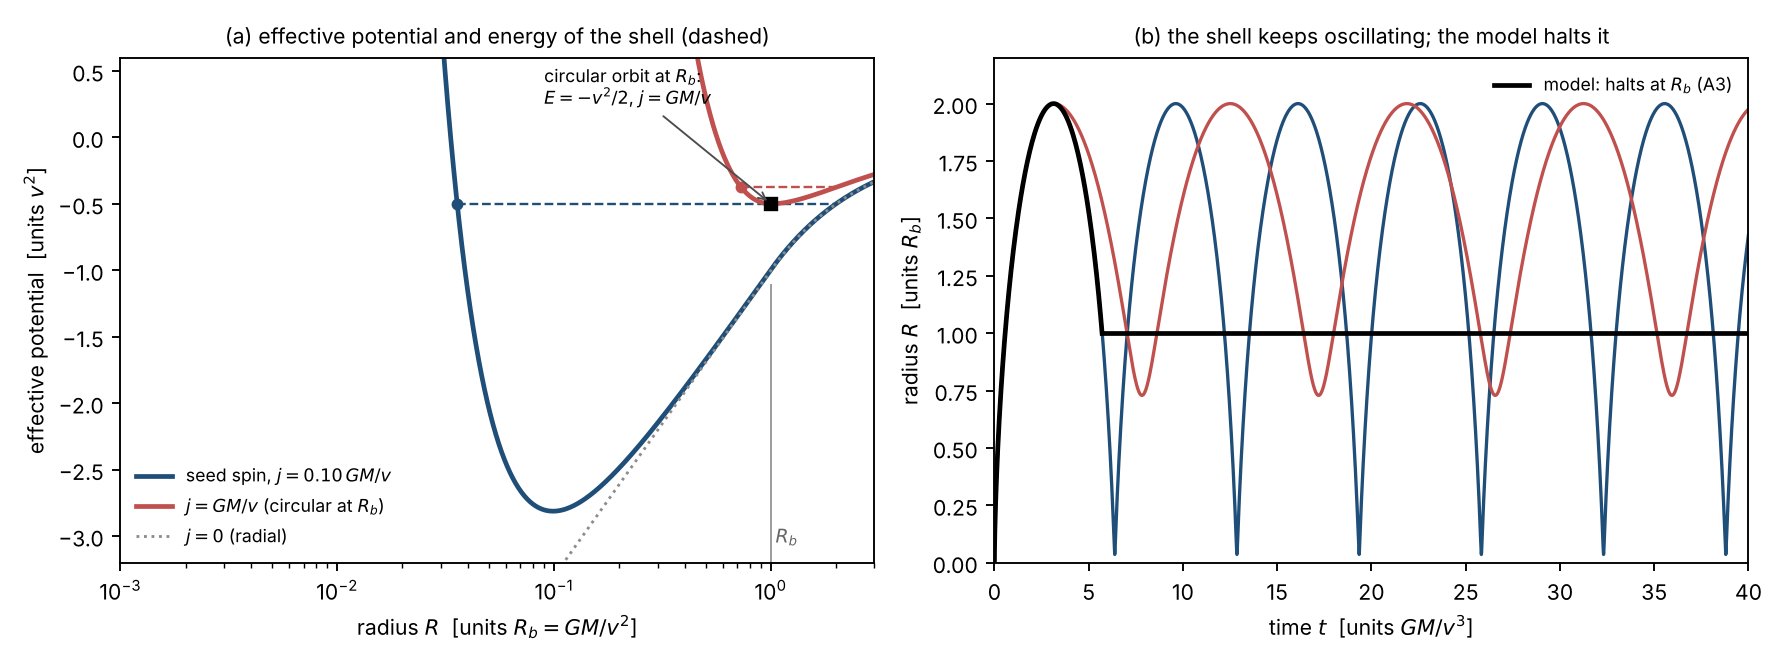
\includegraphics[width=\textwidth]{shell_halt.png}
\caption{One shell (mass $M$, energy $-v^2/2$) falling into the galaxy already
built, taken as a singular isothermal sphere frozen at the moment of arrival; units
$G=M=v=1$, so that $R_b=1$. \textbf{(a)} Effective potential $\Phi+j^2/2R^2$ for
the seed's spin, $j=0.099\,GM/v$ (blue), for $j=GM/v$ (red) and for $j=0$
(dotted), with the shell's energy (dashed) between pericentre (dot) and apocentre.
The square marks the circular orbit at $R_b$, which has exactly the seed's energy.
\textbf{(b)} Radius against time: radial cycloid up to turnaround, then the orbit
with the seed's spin (blue, pericentre $R_b/28$) or with $j=GM/v$ added at turnaround
(red, between $0.73$ and $2\,R_b$); black: the model, which halts the shell at $R_b$.
Script: \texttt{halt.py}, numbers in \texttt{halt\_out.txt}.}
\label{fig:halt}
\end{figure}

\paragraph{What could make the shells settle.}\addcontentsline{toc}{subsection}{What could make the shells settle} Settling requires that individual
particles change their energy and their angular momentum, while the totals are
conserved. For the outermost shell of the example galaxy, the angular momentum per
unit mass must grow from about $500$ to $5050\,{\rm kpc\,km\,s^{-1}}$, and the radial
kinetic energy at the front, $\tfrac12v^2=1800\,({\rm km\,s^{-1}})^2$, must be turned
into tangential motion. Three processes can do this.
\begin{itemize}
\item \emph{Dissipation, for the gas.} Gas falling at $v$ is stopped by an accretion
  shock near the front (cf.\ Bertschinger 1985). A strong shock heats it to
  \begin{equation*}
    T=\frac{3\mu m_p}{16k}\,v^2\simeq4.8\times10^4\,{\rm K}\quad
    (v=60\,{\rm km\,s^{-1}};\ 1.3\times10^5\,{\rm K}\ \text{for}\ 100\,{\rm km\,s^{-1}}),
  \end{equation*}
  with $\mu=0.59$. This is close to the peak of the cooling curve of ionised gas
  near $10^5$\,K, so the gas radiates the energy quickly and settles, with the
  angular momentum it has, into a disc. For the baryons, halting is natural, and the
  energy they radiate is the cooling term of the paper (Sect.~5.4).
\item \emph{Violent relaxation, for the dark matter.} In a collapsing system the
  potential changes on the dynamical time, and a particle's energy is not conserved
  in a time-dependent potential: the rate of change is $\dot E=\partial\Phi/\partial t$
  along its orbit. The energies are thus reshuffled among the particles, with
  changes of order $v^2$ during the collapse (Lynden-Bell 1967). In exact spherical
  symmetry, however, the force is radial and each particle's angular momentum is
  conserved, so violent relaxation alone cannot circularise the orbits.
\item \emph{Torques from departures from spherical symmetry.} A potential with a
  non-spherical part of relative amplitude $\varepsilon$ exerts a tangential force of
  order $\varepsilon\,GM/R^2$, i.e.\ a torque per unit mass $\varepsilon\,GM/R$. Over a
  dynamical time $R/v$ this changes the angular momentum by
  \begin{equation*}
    \Delta j\sim\varepsilon\,\frac{GM}{R}\,\frac{R}{v}=\varepsilon\,\frac{GM}{v}.
  \end{equation*}
  Raising $j$ from $0.1$ to $1\,GM/v$ in a few dynamical times thus requires
  $\varepsilon$ of order 0.3--1: strong, not slight, departures from spherical
  symmetry during the collapse. A cold, nearly radial collapse does produce them: it is
  unstable to bar-like and triaxial distortions (the radial-orbit instability;
  MacMillan et al.\ 2006), and simulated haloes are triaxial with axis ratios of
  about 0.5--0.8. Since the orbits end up oriented at random, each particle can gain
  an angular momentum of order $GM/v$ while the total stays small, as in an Einstein
  cluster; this is why the halo can be nearly isotropic although its net spin is only
  $\lambda\simeq0.035$.
\end{itemize}
None of these exists in a spherical shell code with conserved angular momenta,
which is why the paper's collisionless run (Appendix~H) neither halts its shells nor
forms a core. The $f=1$ run comes closest to the effect of the torques: it gives the
shells the angular momentum of circular orbits, though on top of their energy, and
then yields a nearly flat, isothermal curve, but still no core.

\paragraph{Can star formation and supernovae halt the shells?}\addcontentsline{toc}{subsection}{Can star formation and supernovae halt the shells?} Collapsing gas becomes
dense, forms stars, and the massive ones explode and release energy. One may ask
whether this feedback could stop the infall at the front. The answer is no for the
dark matter, which is what must halt, for four reasons; feedback can, however, stop
the gas and may help to make the core. The numbers below are for the example galaxy
and are computed in \texttt{sf\_numbers.py}.
\begin{enumerate}
\item \emph{Feedback acts on the gas, not on the dark matter.} The energy of a
  supernova, $10^{51}$\,erg, goes into heat and momentum of the surrounding gas.
  Dark matter is collisionless and feels neither pressure nor shocks; it responds only
  to gravity. A dark-matter shell can therefore be affected by feedback only
  indirectly, through a change of the gravitational potential, and only by the
  amount $\dot E=\partial\Phi/\partial t$ along its orbit.
\item \emph{Feedback happens in the wrong place.} Massive stars form in dense, cold
  gas, at hydrogen densities above about $0.1$--$10\,{\rm cm^{-3}}$, i.e.\ in the
  inner disc, within a few kpc of the centre (the example galaxy has
  $r_c=2.44$\,kpc and $R_d\simeq0.67\,r_c\simeq1.6$\,kpc). The shells halt at the
  front, $R_b=84$\,kpc. There the mean density inside the front is 147 times the
  cosmic mean, $1.4\times10^{-27}\,{\rm g\,cm^{-3}}$ for growth ending at $z=0.5$, and
  the local density at the front is a third of that,
  $4.6\times10^{-28}\,{\rm g\,cm^{-3}}$. Even with the full cosmic baryon fraction
  ($0.16$) the gas there has $n_{\rm H}\simeq3\times10^{-5}\,{\rm cm^{-3}}$
  ($8\times10^{-5}$ at $z=1$, $3\times10^{-4}$ at $z=2$): two and a half to five and a half orders of
  magnitude below the threshold for star formation ($0.1/3\times10^{-4}\simeq300$ at the closest). No stars form where the shells
  have to halt.
\item \emph{The indirect effect at the front is small.} Moving gas changes the
  potential at the front by at most the fraction of the mass it moves: if a fraction
  $f$ of the mass inside $R_b$ is carried outside, $\Phi(R_b)=-v^2$ changes by at most
  $f\,v^2$. Our dwarfs hold baryons amounting to only $f\simeq0.017$ of the total mass
  (paper, Sect.~5.4), so a shell's energy changes by at most about $0.02\,v^2$ per
  such event, against the $\tfrac12v^2$ of radial motion that has to be turned into
  tangential motion. Even if all the cosmic baryons, $f=0.16$, were blown out at once,
  the change would be $0.16\,v^2$, and it would still be an energy change: a
  spherically symmetric outflow exerts no torque, so the shell's angular momentum, and
  hence its pericentre at $R_b/28$, would stay the same.
\item \emph{Feedback supplies energy, but the halt needs angular momentum.} As shown
  above, halting a shell at $R_b$ requires no energy at all, only a turn of its
  velocity, i.e.\ an increase of its angular momentum from about $0.1$ to
  $1\,GM/v$. Feedback adds energy: it makes matter less bound and pushes it outwards.
  It is not small: one supernova per $100\,M_\odot$ of stars formed releases
  $(709\,{\rm km\,s^{-1}})^2$ per unit stellar mass, and if a fraction $f_c$ of it
  couples to the matter, the energy gained in units of the binding energy
  $\tfrac12v^2M$ is
  \begin{equation*}
    \epsilon_{\rm fb}=2f_c\Bigl(\frac{709\,{\rm km\,s^{-1}}}{v}\Bigr)^2
    \frac{\Delta M_\star}{M}\simeq280\,f_c\,\frac{\Delta M_\star}{M}
    \quad(v=60\,{\rm km\,s^{-1}}),
  \end{equation*}
  a median of $0.65\,f_c$ for the 79 dwarfs (paper, Table~2). But it is the wrong
  kind of change: it alters how bound the matter is, not how its motion is divided
  between radial and tangential.
\end{enumerate}
What feedback \emph{can} do is different, and both effects are part of the paper's
picture.
\begin{itemize}
\item \emph{It can halt the gas.} Winds driven by supernovae, together with the
  heating by reionisation, can stop or reverse the accretion of gas onto small haloes.
  This is the most likely reason why our dwarfs hold only about a tenth of the cosmic
  baryon fraction, the ``missing baryons'' of the paper (Sect.~8.3). For the baryons,
  feedback can act as a halt; for the dark matter it cannot.
\item \emph{It can make the core.} In the centre, where the baryons are a substantial
  part of the mass (a median 24\% of $V^2$ at $r_c$ in our dwarfs, 12--45\% for the central 68\%), repeated bursts
  that blow gas out and let it fall back make the central potential fluctuate on about
  a dynamical time. Each fluctuation changes the energies of the dark-matter particles
  there; because the particles lose energy while the potential is deep and gain it when
  it is shallow, the net effect over many cycles is to heat the central dark matter and
  push it outwards, turning a cusp into a core (Navarro, Eke \& Frenk 1996; Read \&
  Gilmore 2005; Governato et al.\ 2010; Pontzen \& Governato 2012). In the language of
  the paper, this is a candidate for the settling into a core (A4), not for the halt
  (A3).
\item \emph{It has a price in the model.} Feedback per unit binding energy falls
  steeply with the flat speed, as $v^{-2.5}$, whereas the energy radiated by the
  cooling gas falls only as $v^{-0.6}$ (paper, Sect.~5.4). Cores made by feedback after
  growth would therefore not follow the observed $r_c\propto v$ unless feedback and
  cooling nearly cancel in every dwarf, the fine-tuning of the paper. A feedback core is
  compatible with the model only if it forms during assembly or is regulated by
  cooling.
\end{itemize}
In short, the halting of the dark matter at the front must come from gravity alone:
violent relaxation together with the torques of non-spherical distortions. Star
formation and supernovae, which act later and much further in, can remove most of the
gas and may shape the core, but they cannot stop the infall of the dark matter.

\paragraph{Harmonic motion: what a settled shell does.}\addcontentsline{toc}{subsection}{Harmonic motion: what a settled shell does} Once a shell is close to its
circular orbit, its remaining motion is a set of harmonic oscillations. Three
harmonic equations appear.
\begin{enumerate}
\item \emph{Epicycles about the circular orbit.} Write $R=R_c+X$ with $X\ll R_c$ and
  expand $\Phi_{\rm eff}$, Eq.~\eqref{eq:phieff}, about its minimum $R_c$, where
  $j^2=R_c^3\,{\rm d}\Phi/{\rm d}R$. To first order
  \begin{equation}
    \ddot X+\kappa^2X=0,\qquad
    \kappa^2=\frac{{\rm d}^2\Phi_{\rm eff}}{{\rm d}R^2}\Big|_{R_c}
    =R\frac{{\rm d}\Omega^2}{{\rm d}R}+4\Omega^2,
  \end{equation}
  with $\Omega=v_c/R$ the angular frequency of the circular orbit. The solution is
  \begin{equation}
    X=A\cos(\kappa t+\alpha),\qquad
    \varphi=\Omega t-\frac{2\Omega}{\kappa}\,\frac{A}{R_c}\sin(\kappa t+\alpha),
  \end{equation}
  the second from $\dot\varphi=j/R^2\simeq\Omega(1-2X/R_c)$. In the flat part of the
  curve $\Omega=v/R$ and $\kappa=\sqrt2\,\Omega$: the shell oscillates radially
  $\sqrt2$ times per revolution, so its orbit is a rosette that never closes. At the
  front of the example galaxy $2\pi/\Omega=8.6$\,Gyr and $2\pi/\kappa=6.1$\,Gyr. The
  approximation holds only for $A\ll R_c$; the shells of the seed, with excursions
  from $2R_b$ to $R_b/28$, are far outside it, which is the quantitative sense in
  which they are far from balance.
\item \emph{The harmonic core.} Near the centre of the P18 profile the density is
  constant, $\rho(0)=v^2/(\pi Gr_c^2)$, so the potential is quadratic,
  $\Phi=\tfrac23\pi G\rho(0)R^2+{\rm const}$, and each Cartesian coordinate obeys
  \begin{equation}
    \ddot x=-\omega^2x,\qquad
    \omega^2=\frac{4\pi G\rho(0)}{3}=\frac43\,\frac{v^2}{r_c^2},
  \end{equation}
  with the solution $x=a\cos(\omega t+\alpha)$, $y=b\cos(\omega t+\beta)$,
  $z=c\cos(\omega t+\gamma)$: centred ellipses, all with the same period $2\pi/\omega$
  whatever their size. The circular speed rises linearly, $v_c=\omega R$, which is
  the inner rise $(2/\sqrt3)(v/r_c)R$ of the idealised rotation curve; here
  $\kappa=2\Omega$ and the orbits close. For the example galaxy
  $\omega=28.4\,{\rm km\,s^{-1}\,kpc^{-1}}$ and $2\pi/\omega=216$\,Myr. A particle on
  a radial orbit through the core simply oscillates through the centre with this
  period.
\item \emph{The cycloid itself.} Even the infall of a shell before it halts is a
  harmonic oscillator in disguise. With the time variable $\eta$ of
  Eq.~\eqref{eq:cycloid}, ${\rm d}t=(R/v)\,{\rm d}\eta$, the radial Kepler equation
  becomes
  \begin{equation}
    \frac{{\rm d}^2R}{{\rm d}\eta^2}+R=\frac{GM}{v^2},
  \end{equation}
  whose solution starting at $R=0$ is $R=(GM/v^2)(1-\cos\eta)$: a harmonic oscillation
  about $GM/v^2=R_b$, the halting radius, with amplitude $R_b$. In this variable the
  front is simply the point where the oscillation passes its centre for the second
  time, $\eta=3\pi/2$. A cosmological constant adds a term $\propto R^3$ in this
  equation and breaks the harmonic form, which is why the lag of the front needs the
  perturbation theory of the paper's Appendix~A.
\end{enumerate}

\paragraph{What this means for the model.}\addcontentsline{toc}{subsection}{What this means for the model} Assumptions (A3) and (A4) do not replace
the force balance; they \emph{assume} it. They place every shell at the radius where,
with the seed's energy, gravity and centrifugal force balance, and they assume that
the non-spherical relaxation of a real collapse has turned its radial motion into
tangential motion there. Because energy is conserved in this turn, the energy
bookkeeping of the paper does not depend on how the relaxation proceeds, only on its
end state, just as the virial radius of the classical top-hat model does not depend
on the details of virialisation. What the model cannot explain without such a
mechanism is the core: as the core grows in proportion to $t$, the matter inside it
must keep being rearranged (paper, Appendix~I). Part~II shows what this requires:
nearly isotropic orbits in the core and an energy gain of order $v^2$ for its most
bound matter. Whether non-spherical dynamics can provide this is the open problem
named in the paper's Outlook (Sect.~8.3). The next section tests two simple ways of
breaking the spherical symmetry.

\section{Breaking the symmetry: two numerical experiments}\label{sec:breaking}

Both experiments follow test particles in a fixed, prescribed potential, to which a
non-spherical part is added that grows with time. They do not compute how the
distortion arises; they test what it can do to the orbits once it exists. Units are
$G=v=1$. The scripts and their outputs are part of this package; Part~II
(Sect.~\ref{sec:A4}) measures the results against what the settling requires.

\paragraph{1. A flattening about one axis (\texttt{axi\_test.py},
\texttt{axi\_energy.py}).}\addcontentsline{toc}{subsection}{1.\ A flattening about one axis} Take the flat-curve potential of the settled galaxy and
flatten it along $z$,
\begin{equation}
  \Phi=\frac{v^2}{2}\ln\Bigl(r_s^2+x^2+y^2+\frac{z^2}{q^2}\Bigr),
\end{equation}
with a small softening $r_s=0.01\,R_b$ and an axis ratio $q\le1$ of the potential,
either fixed or decreasing from 1 to $q_{\min}$ over a time $T$. (Below
$q\simeq1/\sqrt2$ this potential would require a negative density at the poles, so
$q=0.7$--0.8 is the strongest flattening possible.) A particle starts at rest at the
turnaround radius $2R_b$, at latitude $20^\circ$, $45^\circ$ or $70^\circ$, and falls
in. Its angular momentum $j$ is measured in units of $GM/v=vR_b$, the value of a
circular orbit at $R_b$.
\begin{itemize}
\item \emph{The flattening turns the infall.} It pulls the particle towards the
  equatorial plane, so radial motion is turned into motion along the meridian. At
  its first pericentre a particle at $45^\circ$ has $j=0.25$ for $q=0.9$, $0.48$ for
  $q=0.8$ and $0.69$ for $q=0.7$; over several orbits $j$ reaches about 1. Particles
  at $+\lambda$ and $-\lambda$ are turned in opposite senses, so the result is a
  dispersion of tangential velocities, not a net rotation.
\item \emph{But the turn is not kept.} In any potential symmetric about the
  $z$-axis, static or not, $\partial\Phi/\partial\varphi=0$, so the component $L_z$
  of each particle's angular momentum is conserved. For the infalling particle
  $L_z=0$, and it stays in its meridional plane. The angular momentum gained there is
  the component perpendicular to that plane, which is not conserved: the orbit
  precesses towards the equator and back, and $j$ swings up and down. The late
  pericentres are $0.02$--$0.18\,R_b$: the orbits keep returning to the centre. Only
  $L_z$ could hold a particle away from the centre for good, and it comes only from
  the seed's spin, which is ten times too small.
\item \emph{A growing flattening adds energy.} As $q$ falls, the potential above and
  below the plane rises under the particle, which gains $0.01$--$0.31\,v^2$
  (\texttt{axi\_energy\_out.txt}); its apocentres stay at $2.0$--$2.3\,R_b$ instead
  of moving in to $R_b$.
\item \emph{A slow growth comes too late.} If $q$ falls from 1 to 0.7 over $10$ or
  $30$ units of $R_b/v$, the first infall gains only $j=0.06$--$0.09$ or
  $0.02$--$0.03$; the turn comes orbits later.
\end{itemize}
A flattening about one axis thus cannot halt the shells at $R_b$. What is needed is a
torque about the axis itself, which requires a distortion without any axis of
symmetry: a triaxial or bar-like shape.

\paragraph{2. A triaxial exponential sphere (\texttt{triax\_core.py}).}\addcontentsline{toc}{subsection}{2.\ A triaxial exponential sphere} The P18
density splits into an isothermal-like part, with $v_c=v(1-e^{-x})$, and an
exponential sphere, $\rho_e=v^2e^{-2R/r_c}/(4\pi Gr_c^2)$, of mass $v^2r_c/4G$, which
carries the whole mass excess $c=\tfrac14$ and a quarter of the central density
(paper, Sect.~2.2). Suppose this central component becomes triaxial. Its potential
is written as a function of the ellipsoidal radius,
\begin{equation}
  \Phi=\Phi_1(r)+\Phi_e(m),\qquad
  m^2=X^2+\frac{Y^2}{p^2}+\frac{Z^2}{q^2},
\end{equation}
where $\Phi_1$ is the potential of the isothermal-like part, $\Phi_e$ that of the
spherical exponential sphere, and $(X,Y,Z)$ are coordinates fixed in the distorted
body, which either stays fixed or tumbles about its short axis at a pattern speed
$\Omega_p$. The axis ratios $p,q$ of this potential grow linearly from 1 to their
final values within $20\,r_c/v$ (0.8\,Gyr for the example galaxy). For $p,q=0.8,0.6$
the total density has axis ratios of about 0.7--0.85 near $r_c$ and is positive
everywhere (\texttt{triax\_density\_check.py}): a moderate distortion. Units are
$r_c=1$ and $R_b=34\,r_c$, the example galaxy ($r_c=2.44$\,kpc, $R_b=84$\,kpc,
$r_c/v=40$\,Myr).

The particles represent the matter accreted early, which in the paper's shell run
fills the core (Appendix~H): 400 nearly radial orbits with apocentres spread
logarithmically between $0.5\,r_c$ and $R_b$, angular momenta $0.05$ times that of a
circular orbit at the apocentre, random orientations and random orbital phases. They
are followed for $300\,r_c/v$, i.e.\ 12\,Gyr. The diagnostic is the time-averaged
density of the particles over the last 4\,Gyr, and its logarithmic slope at
$0.1$--$0.5\,r_c$: a population of radial orbits gives a cusp of slope $-2$; a
population whose velocities have been fully scattered into all directions, at the
same energies, gives a nearly flat core.

\emph{Halting at the front: no.} The exponential sphere has the size $r_c$ and the
mass $v^2r_c/4G$. One passage through it changes the angular momentum by about
$\varepsilon(GM_e/r_c)(r_c/v)\sim\varepsilon\,vr_c/4$, whereas a circular orbit at the
front needs $vR_b$, i.e.\ $y=R_b/r_c$ times more, 34--200. In the runs the orbits
with apocentres beyond $15\,r_c$ keep $j/j_{\rm circ}=0.050$ in every case. A
distortion that is to halt the shells must have the size of the whole galaxy.

\emph{The core: partly.} Table~\ref{tab:triax} and Fig.~\ref{fig:triax} show the
results.
\begin{table}[h]
\centering\small
\caption{Test orbits in P18 with a triaxial exponential sphere after 12\,Gyr. Slope:
logarithmic slope of the time-averaged density at $0.1$--$0.5\,r_c$. $\beta$:
velocity anisotropy inside $r_c$ ($\beta=1$ for radial orbits, 0 for isotropic
ones). $j/j_{\rm circ}$: median for orbits with apocentres below $3\,r_c$ (initially
0.05).}
\label{tab:triax}
\begin{tabular}{lccc}
\hline
case & slope & $\beta$ & $j/j_{\rm circ}$\\
\hline
spherical & $-1.90$ & 0.88 & 0.05\\
triaxial $0.9/0.8$, fixed & $-1.34$ & 0.76 & 0.15\\
triaxial $0.8/0.6$, fixed & $-0.91$ & 0.67 & 0.21\\
$0.8/0.6$, tumbling at $\Omega_p=0.1\,v/r_c$ & $-1.32$ & 0.71 & 0.18\\
$0.8/0.6$, tumbling at $\Omega_p=0.3\,v/r_c$ & $-1.49$ & 0.76 & 0.11\\
$0.9/0.8$, tumbling at $\Omega_p=0.3\,v/r_c$ & $-1.71$ & 0.82 & 0.08\\
\hline
fully scattered, same energies (control) & $-0.39$ & 0.26 & \\
\hline
\end{tabular}
\end{table}
\begin{itemize}
\item \emph{The mechanism.} A triaxial centre deflects the radial orbits that pass
  through it and spreads their motion into all directions; the orbits become chaotic
  (as for triaxial galaxies with a central mass: Gerhard \& Binney 1985; Merritt \&
  Valluri 1996). The energies change by only about $0.003\,v^2$: the experiment
  redistributes angular momentum, it does not heat.
\item \emph{How far it gets.} The strongest case covers about two thirds of the way
  from the radial cusp ($-1.90$) to the fully scattered limit ($-0.39$). Inside about
  $0.1$--$0.2\,r_c$ the profile flattens (Fig.~\ref{fig:triax}), but a core of the
  size $r_c$ is not formed in 12\,Gyr.
\item \emph{Tumbling weakens it.} The faster the distortion rotates, the more its
  pull averages out over an orbit, and the steeper the inner slope stays.
\item \emph{Robustness.} Halving the time step and changing the random sample move the
  slopes by at most 0.07 (\texttt{triax\_control\_out.txt}).
\end{itemize}
\begin{figure}[h]
\centering
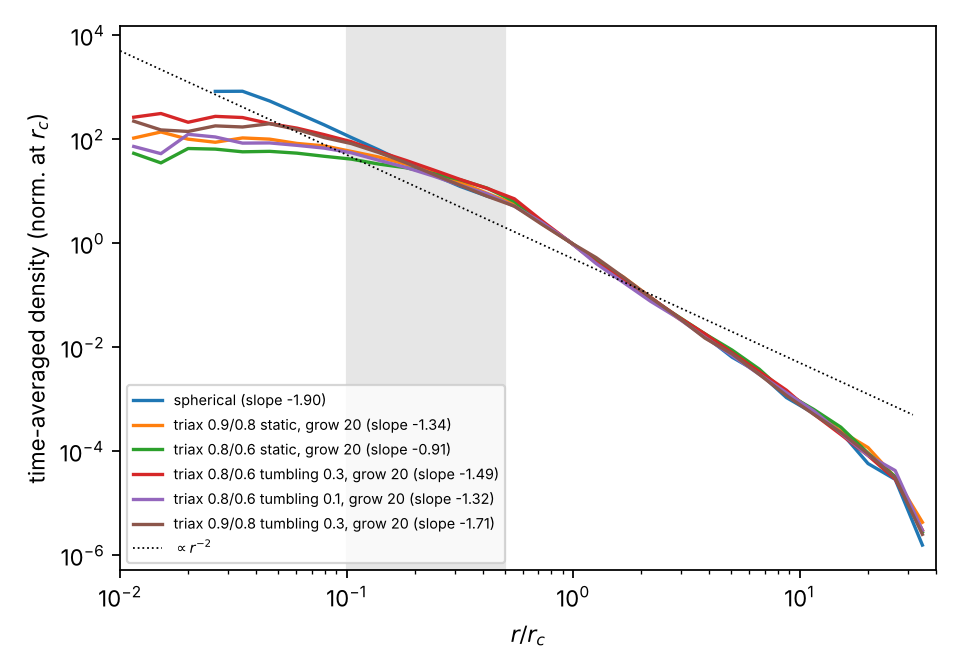
\includegraphics[width=0.8\textwidth]{triax_core.png}
\caption{Time-averaged density of the nearly radial test orbits in P18 with a
triaxial exponential sphere, after 12\,Gyr, normalised at $r_c$; the slopes are fitted
in the grey band. The spherical case keeps the $r^{-2}$ cusp of radial orbits; the
triaxial cases flatten inside about $0.1$--$0.2\,r_c$. The steep fall beyond $r_c$
only reflects the chosen distribution of apocentres.}
\label{fig:triax}
\end{figure}

\emph{The caveat.} The orbits move in a fixed potential that already contains the
core. The experiment therefore tests whether a triaxial core can keep itself cored
against radially infalling matter, not how the core forms; and the exponential sphere
\emph{is} the core. A full answer needs a self-consistent calculation, an $N$-body
run, in which the triaxial shape arises and grows from the infall itself, for example
through the radial-orbit instability.

\paragraph{What the two experiments show.}\addcontentsline{toc}{subsection}{What the two experiments show} They separate the two assumptions of the
paper. The halt at the front (A3) needs torques on the scale of the whole galaxy and
about its own axis, i.e.\ a triaxial or bar-like distortion of the outer halo during
the collapse; a flattening about one axis, or a distortion confined to the centre,
cannot do it. The settling into a core (A4), by contrast, can be helped by a triaxial
centre: it scatters the radial orbits that would otherwise build a cusp, though in
these runs only partly. Both point to the same next step, a three-dimensional
collapse of the paper's seed with its own non-spherical dynamics.


\part{Settling into a core}

\section{The question}

The paper builds a dwarf galaxy from a seed whose shells share the energy
$E=-v^2/2$. Each shell halts at the accretion front, $\Rb=0.175\,vt$, where the
galaxy already built encloses its mass (assumption A3). If the halted matter simply
stayed where it halted, with $M\propto\Rb$, the galaxy would be a \emph{singular
isothermal sphere} (SIS),
\begin{equation}
  \rho_{\rm SIS}=\frac{v^2}{4\pi GR^2},\qquad M_{\rm SIS}(R)=\frac{v^2R}{G},
  \qquad v_c=v,
  \label{eq:sis}
\end{equation}
with a flat rotation curve all the way to the centre and an infinite central
density. The observed dwarfs instead follow P18, which has a core. The paper bridges
the gap with assumption (A4): halted matter settles, conserving mass and energy,
into P18 with the same $v$. It does not say how. The paper's one-dimensional
collisionless calculation (its Appendix~H) shows that spherical shells left to
themselves do not do it: they form a cusp.

Before asking \emph{how} the settling could happen, one can ask \emph{what} it must
achieve. That is the subject of Part~II. We compare the SIS and P18 at three
levels, each more detailed than the one before:
\begin{enumerate}
\item where the mass is (Sect.~\ref{sec:mass});
\item what orbits the mass can be on: first circular orbits
  (Sect.~\ref{sec:circ}), then general orbit populations, described by distribution
  functions (Sect.~\ref{sec:df});
\item how tightly the mass is bound (Sect.~\ref{sec:energy}).
\end{enumerate}
Section~\ref{sec:A4} then spells out what this means for (A4). In Part~II we use
units $G=v=\rc=1$, so that masses are in units of $v^2\rc/G$, energies per unit
mass in $v^2$, and angular momenta per unit mass in $v\rc$; the radius is
$x=R/\rc$.

% ==========================================================================
\section{Where the mass is: P18 as a rearranged SIS}\label{sec:mass}

\subsection{The profile}
The P18 profile is (paper, Eq.~1)
\begin{equation}
  \rho(x)=\frac{v^2u^2}{4\pi GR^2}=\rho_{\rm SIS}(R)\,u(x)^2,
  \qquad u=1-(1-x)\,e^{-x},
  \label{eq:p18}
\end{equation}
with enclosed mass $M=(v^2\rc/G)\,m(x)$, where
\begin{equation}
  m(x)=\int_0^xu^2\,\dd x'=x(1-e^{-x})^2+\tfrac14\bigl[1-(1+2x+2x^2)e^{-2x}\bigr].
  \label{eq:m}
\end{equation}
Equation~\eqref{eq:p18} already says the essential thing: \emph{P18 is the SIS
multiplied by $u^2$}. All the information about the core is in the factor $u^2$.

\subsection{A useful rewriting of $u$}
Writing $u$ as $1+(x-1)e^{-x}$ makes its behaviour obvious:
\begin{itemize}
\item for $x<1$ the correction $(x-1)e^{-x}$ is negative: $u<1$, so P18 has
  \emph{less} density than the SIS;
\item at $x=1$ it vanishes: $u(1)=1$ \emph{exactly}, so P18 and the SIS have the
  same density at $R=\rc$;
\item for $x>1$ it is positive: $u>1$, P18 has \emph{more} density than the SIS.
  The correction is largest where its derivative, $(2-x)e^{-x}$, vanishes, at $x=2$,
  where $u^2=(1+e^{-2})^2=1.289$; beyond that it decays exponentially.
\end{itemize}
The core radius thus has a precise meaning: $\rc$ is the radius at which P18
crosses the singular isothermal sphere of the same $v$ (Fig.~\ref{fig:summary}a).

\subsection{How much mass is moved}
The mass that P18 lacks inside $\rc$, compared with the SIS, is
\begin{equation}
  \int_0^1(1-u^2)\,\dd x=1-m(1)=0.520,
\end{equation}
and the mass it has in addition outside $\rc$ is
\begin{equation}
  \int_1^\infty(u^2-1)\,\dd x=0.770.
\end{equation}
The difference, $0.770-0.520=0.250$, is the mass excess $c=\int_0^\infty(u^2-1)\,
\dd x=\tfrac14$ of the paper (Sect.~2.2). The enclosed masses become equal again at
$x=3.29$, where $m(x)=x$ (Table~\ref{tab:mass}).

\begin{table}[h]
\centering\small
\caption{Enclosed mass of P18 and of the SIS of the same $v$ (units $v^2\rc/G$).
The last column is the mass that P18 still lacks inside $x$.}
\label{tab:mass}
\begin{tabular}{rrrr}
\toprule
$x=R/\rc$ & $m(x)$ (P18) & $x$ (SIS) & $x-m(x)$\\
\midrule
0.1 & 0.0012 & 0.1 & 0.099\\
0.3 & 0.026 & 0.3 & 0.274\\
0.5 & 0.097 & 0.5 & 0.403\\
1 & 0.480 & 1 & 0.520\\
2 & 1.686 & 2 & 0.314\\
3 & 2.943 & 3 & 0.057\\
5 & 5.182 & 5 & $-0.182$\\
10 & 10.249 & 10 & $-0.249$\\
\bottomrule
\end{tabular}
\end{table}

Two remarks help to read these numbers.
\begin{itemize}
\item \emph{The rearrangement is small.} A galaxy with core ratio $y=\Rb/\rc$
  contains the mass $y\,v^2\rc/G$ inside its front. The mass taken out of the core is
  therefore a fraction $0.52/y$ of the galaxy: 1.5\% for the example galaxy of the
  paper ($y=34.4$), 0.5\% for $y=100$ and 0.26\% for $y=200$. The core is a small
  rearrangement in the centre of an otherwise isothermal galaxy.
\item \emph{The mass excess is a compaction.} Far out $m\to x+\tfrac14$, so a P18
  galaxy holding the mass $M$ has its front at $\Rb=GM/v^2-\rc/4$: a quarter of a
  core radius inside the front of the SIS with the same mass. In words: the matter
  removed from the core is put back just outside it, and a little more, and the
  galaxy as a whole is slightly more compact.
\end{itemize}

\subsection{A remark on the very centre}
Near the centre $u=2x-\tfrac32x^2+\dots$, so
\begin{equation}
  \frac{\rho}{\rho(0)}=\Bigl(\frac{u}{2x}\Bigr)^2=1-\tfrac32x+O(x^2),
  \qquad \rho(0)=\frac{v^2}{\pi G\rc^2}.
  \label{eq:centre}
\end{equation}
The density falls \emph{linearly} with radius: its logarithmic slope goes to zero,
so P18 has a core in the usual sense, but its slope ${\rm d}\rho/{\rm d}R$ does not.
The Burkert profile, $\rho\propto1/[(1+x)(1+x^2)]$, shares this property; the
pseudo-isothermal sphere, $\rho\propto1/(1+x^2)$, does not. We shall meet the
consequence in Sect.~\ref{sec:iso}.

% ==========================================================================
\section{Circular orbits: the angular momentum of each shell}\label{sec:circ}

The halting rule of the paper places each shell, in the idealisation, on a circular
orbit. A circular orbit at $R$ has $v_c^2=GM(R)/R$ and specific angular momentum
\begin{equation}
  j=Rv_c=\sqrt{GM(R)\,R}=\frac{GM(R)}{v_c(R)}.
  \label{eq:jcirc}
\end{equation}
In the SIS, $v_c=v$ everywhere and each shell has $j=GM/v$. In P18 the shell
enclosing the same mass sits at a different radius, and $j=GM/v_c$ with the smaller
circular speed of the core. In units of the SIS value,
\begin{equation}
  \frac{j_{\rm P18}}{GM/v}=\frac{v}{v_c(R)}=\sqrt{\frac{x}{m(x)}},
\end{equation}
which is 1.44 at $\rc$, 3.4 at $0.3\,\rc$ and 9.2 at $0.1\,\rc$
(Table~\ref{tab:j}, Fig.~\ref{fig:summary}b). The seed gives each shell, at
turnaround, $j=\sqrt2\lambda vR_{\rm ta}=2\sqrt2\lambda\,GM/v=0.099\,GM/v$ for the
median spin $\lambda=0.035$ (paper, Appendix~H).

\begin{table}[h]
\centering\small
\caption{Angular momentum needed by a shell on a circular orbit in P18.}
\label{tab:j}
\begin{tabular}{rrrr}
\toprule
$x$ & $v_c/v$ & $j/(GM/v)$ & $j/j_{\rm seed}$\\
\midrule
0.1 & 0.109 & 9.16 & 92\\
0.3 & 0.294 & 3.40 & 34\\
0.5 & 0.442 & 2.27 & 23\\
1 & 0.693 & 1.44 & 15\\
2 & 0.918 & 1.09 & 11\\
3 & 0.991 & 1.01 & 10\\
$\ge5$ & 1.01--1.02 & 0.98--0.99 & 10\\
\bottomrule
\end{tabular}
\end{table}

Read literally, this says: in the flat part every shell needs ten times the seed's
angular momentum, and in the core even more, up to a hundred times. The seed does the
opposite: its $j\propto M$ is smallest for the innermost, earliest shells. This is the
``ten times too little'' of Sect.~\ref{sec:why}, sharpened in the core.

But this reading assumes circular orbits, and nothing forces them. A rotation curve
measures only the enclosed mass, not the orbits that carry it. The same density can
be carried by circular orbits, by radial orbits, or by anything in between. To find
out which orbits P18 \emph{allows}, we need distribution functions.

% ==========================================================================
\section{Orbit populations: distribution functions}\label{sec:df}

\subsection{What a distribution function is}
A collisionless system is described by its distribution function $f(\mathbf
x,\mathbf v)$: the mass per unit volume of phase space, so that $f\,\dd^3x\,
\dd^3v$ is the mass in a small cell of positions and velocities. The density is
$\rho(\mathbf x)=\int f\,\dd^3v$.

In a steady state, $f$ is constant along every orbit (Liouville's theorem), so it
can depend on $\mathbf x$ and $\mathbf v$ only through quantities that are conserved
along orbits. This is the \emph{Jeans theorem}. In a static spherical potential
$\Phi(r)$ the conserved quantities are the energy per unit mass
$E=\Phi(r)+\tfrac12v^2$ and the angular momentum vector $\mathbf L$; for a
spherical system without net rotation, $f=f(E,L)$ with $L=|\mathbf L|$.

A function of two variables cannot be recovered from a density, which is a function
of one. So we must choose a one-parameter family of orbit populations, and ask for
which members $f\ge0$ everywhere. A negative $f$ means a negative mass somewhere in
phase space: that population of orbits cannot produce the density. We use two
families:
\begin{itemize}
\item \emph{isotropic}, $f=f(E)$: velocities point in all directions with equal
  probability at every point;
\item \emph{Osipkov--Merritt} (Osipkov 1979; Merritt 1985), $f=f(Q)$ with
  $Q=E+L^2/(2r_a^2)$: isotropic well inside the \emph{anisotropy radius} $r_a$,
  increasingly radial outside it.
\end{itemize}
The potential is that of P18 itself, $\dd\Phi/\dd r=GM(r)/r^2=m(x)/x^2$ in our
units, with $\Phi(0)\equiv0$. Since $m\to x+\tfrac14$, far out
$\Phi\to\ln x+0.134-1/(4x)$: the potential grows without bound, every orbit is
bound, and $E$ runs from $\Phi(0)=0$ to $\infty$.

\subsection{Eddington's inversion, step by step}\label{sec:edd}
For an isotropic population at radius $r$, the velocities with speeds between $v$
and $v+\dd v$ fill a spherical shell of volume $4\pi v^2\dd v$ in velocity space.
With $E=\Phi+\tfrac12v^2$ we have $v\,\dd v=\dd E$ and $v=\sqrt{2(E-\Phi)}$, so
\begin{equation}
  \rho(r)=4\pi\int_0^\infty f\,v^2\dd v
  =4\pi\int_{\Phi(r)}^\infty f(E)\,\sqrt{2(E-\Phi)}\;\dd E.
  \label{eq:rhoE}
\end{equation}
The right-hand side depends on $r$ only through $\Phi(r)$. Since $\Phi$ grows
monotonically with $r$, we may regard $\rho$ as a function of $\Phi$. Differentiating
with respect to $\Phi$ (the boundary term vanishes because $\sqrt{E-\Phi}=0$ at the
lower limit),
\begin{equation}
  \frac{\dd\rho}{\dd\Phi}=-2\sqrt2\,\pi\int_\Phi^\infty\frac{f(E)\,\dd E}
  {\sqrt{E-\Phi}}.
  \label{eq:abel1}
\end{equation}
This is an \emph{Abel integral equation}: the known function
$g(\Phi)=-(\dd\rho/\dd\Phi)/(2\sqrt2\pi)$ equals $\int_\Phi^\infty
f(E)\,(E-\Phi)^{-1/2}\dd E$. Abel showed that it has the unique solution
\begin{equation}
  f(E)=-\frac1\pi\,\frac{\dd}{\dd E}\int_E^\infty\frac{g(\Phi)\,\dd\Phi}{\sqrt{\Phi-E}}.
\end{equation}
(You can check it by inserting the equation for $g$ and exchanging the order of
integration; the inner integral is $\int_E^{E'}[(\Phi-E)(E'-\Phi)]^{-1/2}\dd\Phi=\pi$.)
Substituting $g$, and then $\Phi=E+s$ so that the $E$-derivative can be taken inside
the integral,
\begin{equation}
  \boxed{\;f(E)=\frac{1}{2\sqrt2\,\pi^2}\int_E^\infty
  \frac{\dd^2\rho}{\dd\Phi^2}\,\frac{\dd\Phi}{\sqrt{\Phi-E}}\;}
  \label{eq:edd}
\end{equation}
This is \emph{Eddington's formula} (Eddington 1916; Binney \& Tremaine 2008,
Sect.~4.3), in the form suited to a potential without an escape energy. A useful
test: for the SIS, $\rho\propto e^{-2\Phi/v^2}$, so $\dd^2\rho/\dd\Phi^2=4\rho/v^4$,
and Eq.~\eqref{eq:edd} gives $f\propto e^{-2E/v^2}$: a Maxwellian velocity
distribution with dispersion $\sigma^2=v^2/2$, the same at every radius. This is
why the SIS is called isothermal.

For P18 we compute $\dd^2\rho/\dd\Phi^2$ analytically from Eqs.~\eqref{eq:p18} and
\eqref{eq:m}, using
$\dd/\dd\Phi=(\dd\Phi/\dd r)^{-1}\dd/\dd r$, and evaluate Eq.~\eqref{eq:edd}
numerically with the substitution $\Phi=E+t^2$, which removes the integrable
singularity at $\Phi=E$. As a check, the density rebuilt from $f$ with
Eq.~\eqref{eq:rhoE} agrees with P18 to 0.03\% from $10^{-3}$ to $100\,\rc$.

\subsection{The isotropic P18}\label{sec:iso}
The result (Fig.~\ref{fig:df}a):
\begin{itemize}
\item \emph{$f(E)>0$ everywhere}: P18 can be made of isotropic orbits.
\item \emph{Outer energies}: for orbits that live beyond about $4\rc$, $f$ is within
  8\% of the isothermal $f\propto e^{-2E/v^2}$ of the SIS with the same far field.
  Outside the core, P18 is an isothermal sphere in phase space as well.
\item \emph{Inner energies}: towards the bottom of the potential $f$ rises as
  \begin{equation}
    f(E)\simeq\frac{0.0105}{E-\Phi(0)}\qquad\bigl(\text{units }G=v=\rc=1\bigr).
  \end{equation}
  This is the phase-space signature of the linear density decline,
  Eq.~\eqref{eq:centre}. Near the centre $\Phi=\tfrac23x^2$, so
  $\rho\simeq\rho(0)[1-\tfrac32(\tfrac32\Phi)^{1/2}]$ and
  $\dd^2\rho/\dd\Phi^2=\tfrac14(\tfrac32)^{3/2}\rho(0)\,\Phi^{-3/2}$; inserted in
  Eq.~\eqref{eq:edd}, with $\int_E^\infty\Phi^{-3/2}(\Phi-E)^{-1/2}\dd\Phi=2/E$,
  this gives $f=(\tfrac32)^{3/2}\rho(0)/(4\sqrt2\pi^2E)$, i.e.\ the coefficient
  0.0105 found numerically. The divergence is integrable and harmless: the density
  stays finite.
\end{itemize}

\subsection{How radial may the orbits be?}\label{sec:om}
Matter arrives by radial infall, so the natural question is how much of the radial
character it may keep. In the Osipkov--Merritt family $f$ depends on
$Q=E+L^2/(2r_a^2)$. At radius $r$, with radial and tangential velocities $v_r$ and
$v_t$, $L=rv_t$ and
\begin{equation}
  Q=\Phi+\tfrac12v_r^2+\tfrac12v_t^2\Bigl(1+\frac{r^2}{r_a^2}\Bigr).
\end{equation}
Stretching the tangential velocities, $v_t'=v_t(1+r^2/r_a^2)^{1/2}$, turns $Q$ into
an ordinary energy, $Q=\Phi+\tfrac12(v_r^2+v_t'^2)$, while the volume element of
velocity space shrinks by the factor $1+r^2/r_a^2$. Hence
\begin{equation}
  \Bigl(1+\frac{r^2}{r_a^2}\Bigr)\rho(r)
  =4\pi\int_\Phi^\infty f(Q)\,\sqrt{2(Q-\Phi)}\;\dd Q:
\end{equation}
exactly Eq.~\eqref{eq:rhoE}, with $\rho$ replaced by the ``augmented density''
$\rho_Q=(1+r^2/r_a^2)\rho$. So $f(Q)$ follows from Eddington's formula applied to
$\rho_Q$. The velocity anisotropy,
\begin{equation}
  \beta(r)=1-\frac{\sigma_t^2}{2\sigma_r^2}=\frac{r^2}{r^2+r_a^2},
\end{equation}
is 0 (isotropic) at the centre and tends to 1 (purely radial) far outside $r_a$.

Small $r_a$ means radial orbits far in. We find (Fig.~\ref{fig:df}b):
\begin{itemize}
\item for $r_a\ge0.865\,\rc$ the function $f(Q)$ is positive everywhere;
\item for smaller $r_a$ it becomes negative, always at the energies of orbits around
  the core: for $r_a=0.7\,\rc$ at energies of circular orbits between $0.44$ and
  $1.3\,\rc$, for $r_a=0.5\,\rc$ between $0.25$ and $1.5\,\rc$.
\end{itemize}
The most radial P18 of this family thus has $r_a=0.87\,\rc$, with
\begin{equation}
  \beta=0.57\ \text{at}\ \rc,\qquad0.84\ \text{at}\ 2\rc,\qquad
  0.97\ \text{at}\ 5\rc
\end{equation}
(Fig.~\ref{fig:summary}c). Outside about $2\rc$ the orbits may be almost purely
radial; inside $\rc$ they must be close to isotropic.

This is an instance of a general theorem. For a density $\rho\propto r^{-\gamma}$ at
the centre, a positive distribution function requires $\gamma\ge2\beta(0)$ (An \&
Evans 2006; proved for wide classes of models by Ciotti \& Morganti 2010). A cusp
can be built from radial orbits, but a core, $\gamma=0$, cannot have radially biased
orbits at its centre. Purely radial orbits, which all pass through the centre,
always produce $\rho\propto r^{-2}$ there; this is why the radial infall of the
paper's shell run fills the centre with a cusp.

\begin{figure}[t]
\centering
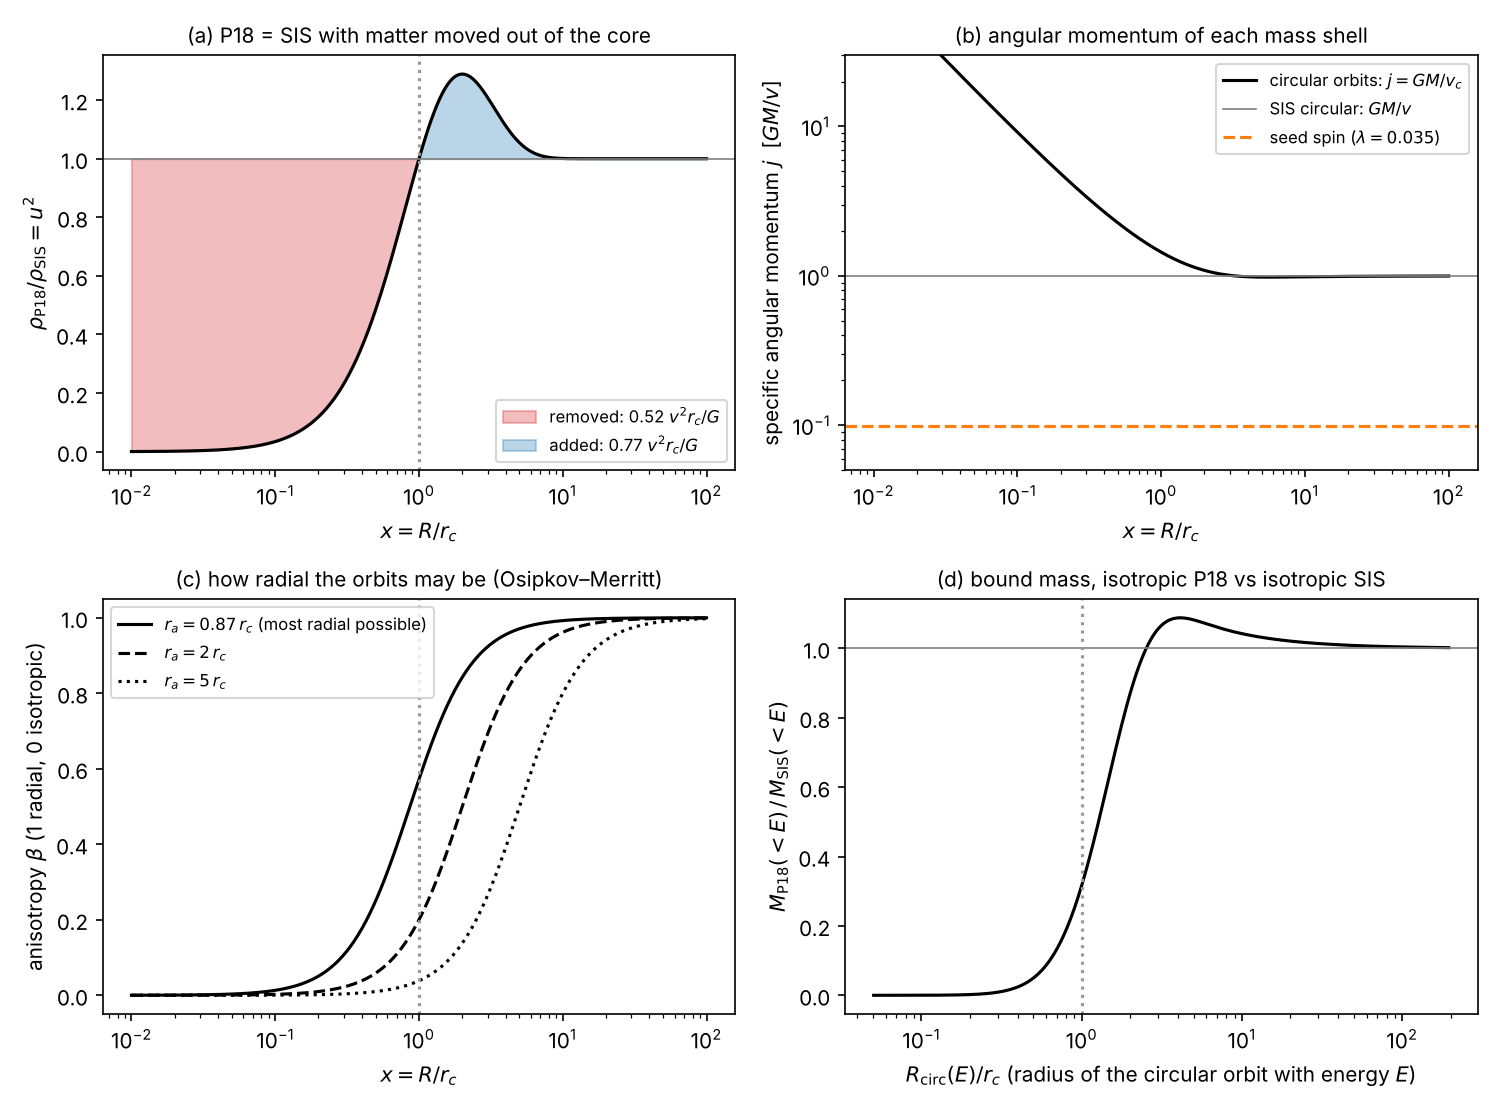
\includegraphics[width=\textwidth]{p18_inverse.png}
\caption{What turns the SIS into P18 (units $G=v=\rc=1$). (a)~Density ratio
$u^2$: P18 lacks $0.52\,v^2\rc/G$ inside $\rc$ (red) and has $0.77$ more outside
(blue). (b)~Specific angular momentum of a shell on a circular orbit, in units of
$GM/v$, compared with the SIS and with the seed's spin. (c)~Velocity anisotropy of
Osipkov--Merritt models; $r_a=0.87\,\rc$ is the most radial one with a positive
distribution function. (d)~Mass with energy below $E$ in the isotropic P18,
relative to the isotropic SIS with the same far field, against the radius of the
circular orbit of that energy. Script: \texttt{p18\_inverse\_fig.py}.}
\label{fig:summary}
\end{figure}

\begin{figure}[t]
\centering
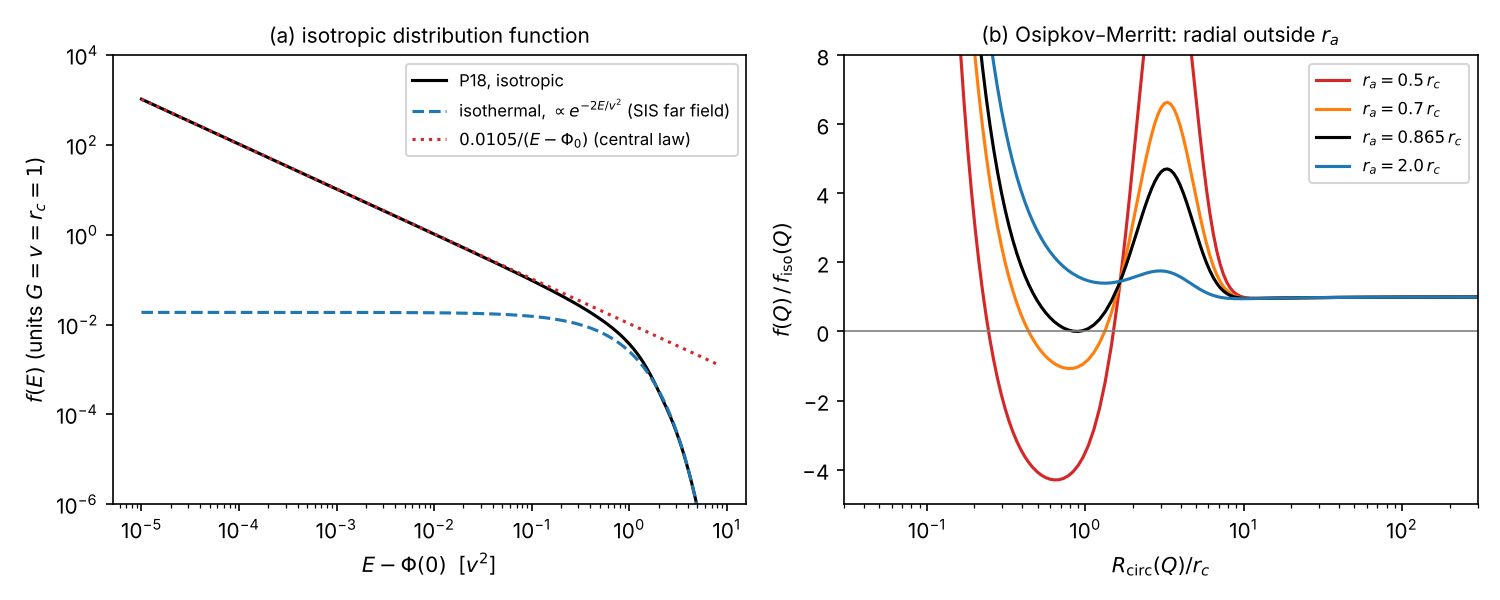
\includegraphics[width=\textwidth]{p18_df.png}
\caption{(a)~Isotropic distribution function of P18 (solid), the isothermal one of the
SIS with the same far field (dashed) and the central law $0.0105/(E-\Phi_0)$
(dotted). (b)~Osipkov--Merritt distribution functions, relative to the isothermal
one, against the radius of the circular orbit of energy $Q$: for $r_a<0.865\,\rc$
they become negative at the energies of the core. Script:
\texttt{p18\_df\_fig.py}.}
\label{fig:df}
\end{figure}

% ==========================================================================
\section{How tightly the mass is bound}\label{sec:energy}

The distribution function also tells how the mass is distributed in energy. The
phase-space volume with energies between $E$ and $E+\dd E$ is $g(E)\,\dd E$, with the
\emph{density of states}
\begin{equation}
  g(E)=\int\dd^3x\int\dd^3v\;\delta\bigl(E-\Phi-\tfrac12v^2\bigr)
  =16\pi^2\int_0^{r_E}r^2\sqrt{2(E-\Phi(r))}\;\dd r,
\end{equation}
where $\Phi(r_E)=E$; the factor $4\pi v=4\pi\sqrt{2(E-\Phi)}$ comes from
$\dd^3v=4\pi v^2\dd v$ and $\dd E=v\,\dd v$. The mass per unit energy is
$N(E)=f(E)\,g(E)$, and the mass bound more tightly than $E$ is
$M(<E)=\int^E N\,\dd E'$.

To compare P18 with the SIS we must put both on the same energy scale. We take both
isotropic and match their potentials far out, where the two galaxies are the same
(the SIS potential is $\ln x+0.134$). To give each energy a meaning, we label it by
the radius $R_{\rm circ}(E)$ of the circular orbit of that energy in P18.
Table~\ref{tab:energy} and Fig.~\ref{fig:summary}d show the result.

\begin{table}[h]
\centering\small
\caption{Mass bound more tightly than $E$, isotropic P18 and isotropic SIS with the
same far field (units $v^2\rc/G$).}
\label{tab:energy}
\begin{tabular}{rrrrr}
\toprule
$E-\Phi(0)$ & $R_{\rm circ}(E)/\rc$ & $M_{\rm P18}(<E)$ & $M_{\rm SIS}(<E)$ & ratio\\
\midrule
0.10 & 0.32 & 0.006 & 0.527 & 0.011\\
0.30 & 0.62 & 0.060 & 0.641 & 0.094\\
0.51 & 0.90 & 0.200 & 0.792 & 0.25\\
1.00 & 1.61 & 0.904 & 1.294 & 0.70\\
1.50 & 2.58 & 2.15 & 2.13 & 1.01\\
1.98 & 4.0 & 3.76 & 3.45 & 1.09\\
2.98 & 10.6 & 9.77 & 9.39 & 1.04\\
3.98 & 28.6 & 25.9 & 25.6 & 1.015\\
5.99 & 211 & 189.7 & 189.3 & 1.002\\
\bottomrule
\end{tabular}
\end{table}

The SIS has matter at all energies down to $-\infty$, its infinitely deep centre.
P18 has none below $\Phi(0)$, and little just above it: only a quarter as much
matter as the SIS is bound more tightly than a circular orbit at $0.9\,\rc$, and 1\%
as much more tightly than one at $0.3\,\rc$. The missing matter reappears at the
energies of orbits at 2.6--30\,$\rc$, with up to 9\% more than in the SIS. In the
language of energy, the core is the \emph{absence of the most bound matter}: the
matter that in an SIS would sit deep in the central cusp is, in P18, on orbits of a
few core radii.

One caution. The energy distribution depends on the orbits, not only on the density;
the comparison here is between two \emph{isotropic} systems. With different orbit
populations the numbers change, but not the conclusion that the energies of the
inner matter must be raised: no rearrangement of orbits at fixed energies can remove
the matter from the bottom of the SIS well, because a particle cannot rise above
its own energy.

% ==========================================================================
\section{What this means for assumption (A4)}\label{sec:A4}

Assumption (A4) states that halted matter settles, conserving mass and energy, into
P18 with the same $v$. The results above turn this into a list of concrete
requirements, and also show what (A4) does \emph{not} require.

\subsection{What (A4) requires}
\begin{enumerate}
\item \emph{A small rearrangement of mass.} Compared with the isothermal galaxy the
  halted matter would form, $0.52\,v^2\rc/G$ must be moved from inside $\rc$ to
  between $\rc$ and about $5\rc$, together with a compaction of the whole galaxy by
  $\rc/4$ (the mass excess). This is 0.3--1.5\% of the galaxy's mass for core ratios
  $y=34$--200. (A4) concerns the innermost percent of the galaxy, not the galaxy as
  a whole.

\item \emph{Isotropic orbits in the core.} Inside $\rc$ the orbits must be close to
  isotropic: in the Osipkov--Merritt family $\beta\le0.57$ at $\rc$ and $\beta\to0$
  at the centre, and by the theorem of An \& Evans no positive distribution function
  has radially biased orbits at the centre of a core. Radial infall delivers the
  opposite, $\beta\simeq1$. The infalling matter must therefore have its velocities
  turned into all directions \emph{before or while} it passes through the core.
  The angular momentum this needs is of the core's own scale, $j\sim v\rc$, not
  $GM/v$ at the front: the inner matter must miss the centre by about a core radius.

\item \emph{An energy lift.} The most bound matter of the isothermal galaxy must be
  raised by energies of order $v^2$ (Table~\ref{tab:energy}: from below the circular
  energy at $0.3\,\rc$ to that of orbits at a few $\rc$, a difference of more than
  $v^2$). A collisionless particle changes its energy only through a potential that
  changes in time: along its orbit $\dd E/\dd t=\partial\Phi/\partial t$. A static
  distortion, however strong, can turn velocities and redistribute angular momentum
  but cannot lift energies. (A4) therefore requires a time-dependent potential in
  the centre: a collapse that is still violently relaxing, a tumbling or oscillating
  bar, fluctuations driven by gas, or sinking clumps.

\item \emph{Continuity during growth.} During growth the core grows as
  $\rc\propto t$, and the mass that must be held out of the core,
  $0.52\,v^2\rc/G$, grows with it. The rearrangement is not a single event: matter
  accreted earlier, which settled when the core was smaller, must be lifted again
  and again as the core sweeps over it. This is the flow of matter in a growing core
  described in the paper's Appendix~I, now with its energy requirement attached.

\item \emph{Mostly an internal transfer of energy.} (A4) adds no energy from
  outside: the settled galaxy has the energy of the seed. The paper's core equation
  does this global bookkeeping; for the example galaxy the core term is $-0.0082$ of
  the binding energy $\tfrac12v^2M$ and balances the spin ($+0.0037$) and $\Lambda$
  ($+0.0045$) terms (paper, Table~2). The local lift of item~3 is larger: of order
  $0.5\,v^2\rc/G$ of matter raised by about $v^2$, i.e.\ some $0.5\,v^4\rc/G$, about
  3\% of the binding energy $\tfrac12v^2\cdot y\,v^2\rc/G$ for $y=34$. The net
  energy of the core is thus only a part of what the inner matter must gain; the rest
  must come from matter elsewhere in the galaxy that becomes more bound. This is the
  ``internal transfer, not net'' of the paper's Table~2, here traced to where it
  must go. The estimate is rough; a mechanism should be judged by whether it moves
  energy \emph{inwards to the core matter} at about this rate.
\end{enumerate}

\subsection{What (A4) does not require}
\begin{itemize}
\item \emph{Circular orbits at the front.} The flat part of P18, outside about
  $2\rc$, can be carried by nearly radial orbits (Sect.~\ref{sec:om}). The
  ``tenfold'' angular momentum of Table~\ref{tab:j} is the price of the idealised
  picture with circular orbits, not of the density. For the density, what matters
  outside the core is the distribution of the orbits' energies, i.e.\ where they turn
  around, not their angular momenta. Whether the seed delivers exactly the energies
  for $\rho\propto r^{-2}$ is a separate question; the paper's shell run says: not
  quite, its curve falls from $v_c^2=1.54\,v^2$ at $0.1\,\Rb$ to $0.86\,v^2$ at
  $\Rb$ (Appendix~H).
\item \emph{A net rotation.} Isotropy needs angular momenta in all directions, which
  cancel; the net spin can stay at the seed's $\lambda\simeq0.035$.
\item \emph{Any change of the outer galaxy.} Beyond about $7\rc$ P18 and the SIS
  agree to about 1\% in density ($u^2-1\simeq2(x-1)e^{-x}$), and in phase space the
  isotropic P18 is within 8\% of the isothermal distribution function for orbits
  beyond about $4\rc$.
\end{itemize}

\subsection{The candidate mechanisms, measured against these requirements}
\begin{itemize}
\item \emph{Violent relaxation of a non-spherical collapse.} It provides both the
  time-dependent potential (item~3) and the turning of velocities (item~2). In
  exact spherical symmetry it fails, as the paper's shell run shows: the angular
  momenta are conserved and the radial orbits fill the centre. With the radial-orbit
  instability, which makes a cold collapse bar-like or triaxial, it is the most
  natural candidate.
\item \emph{A triaxial centre.} The test-particle experiment of
  Sect.~\ref{sec:breaking} gave isotropy only in part ($\beta=0.67$ inside $\rc$, against $\beta\le
  0.57$ at $\rc$ and $\beta\to0$ at the centre required here) and almost no energy
  change ($|\Delta E|\simeq0.003\,v^2$), because its potential was static apart from
  a slow growth. Its partial flattening of the cusp, to a slope of $-0.9$, is what
  items~2 and~3 lead one to expect from turning velocities without lifting energies.
  A tumbling or growing distortion that changes on the dynamical time of the core,
  about 200\,Myr in the example galaxy, would act on both.
\item \emph{Sinking clumps.} Substructure that sinks by dynamical friction transfers
  its orbital energy to the central dark matter (El-Zant, Shlosman \& Hoffman 2001):
  an energy lift (item~3) paid from within the galaxy (item~5).
\item \emph{Feedback.} Repeated gas outflows make the central potential fluctuate and
  lift the central dark matter (Pontzen \& Governato 2012): items~2 and~3. Its
  difficulty in the model is the scaling with $v$ (paper, Sect.~5.4;
  Sect.~\ref{sec:why}).
\item \emph{Self-interacting dark matter.} Collisions isotropise the velocities and
  conduct energy outwards into the core: items~2 and~3 at once, and the result is
  close to isothermal, as P18 is outside the core. Its core scales with $v$ in a way
  set by the cross-section (paper, Sect.~8.2).
\end{itemize}

\subsection{What a simulation should look for}
These requirements can be checked directly in a simulation of the paper's seed, or
in any simulation of a cored dwarf:
\begin{itemize}
\item the velocity anisotropy of the dark matter: close to isotropic inside $\rc$,
  allowed to be radial beyond about $2\rc$;
\item the energy distribution $M(<E)$ of the inner matter, compared with
  Table~\ref{tab:energy};
\item the time dependence of the central potential while the core grows, and
  whether the energy gained by the inner matter matches the energy lost by the
  matter just outside.
\end{itemize}

% ==========================================================================
\section{Limits of this note}\label{sec:limits}
\begin{itemize}
\item Part~I follows the seed only until each shell halts; the halting itself is
  the assumption (A3), and a one-dimensional collisionless calculation in which the
  shells are not halted forms a cusp instead (paper, Sect.~8.1 and Appendix~H). The
  test-particle experiments of Sect.~\ref{sec:breaking} use fixed potentials and are
  not self-consistent.
\item Part~II concerns only the \emph{end state}: what P18 is in phase space and
  how it differs from the SIS. It shows what a settling mechanism must achieve, not
  that the seed's collapse achieves it.
\item The potential is that of P18 alone. In real dwarfs the baryons contribute a
  median 24\% of $V^2$ at $\rc$ (paper, Appendix~E); for the total-matter profile of
  the paper this does not matter, but the orbits of the dark matter alone live in the
  total potential.
\item Two families of distribution functions were used. Others exist; the theorem
  $\gamma\ge2\beta(0)$ and the energy argument of Sect.~\ref{sec:energy} hold beyond
  them, the number $r_a\ge0.87\,\rc$ does not.
\item The energy comparison of Sect.~\ref{sec:energy} assumes isotropy for both
  systems; the statement that inner energies must be raised does not.
\end{itemize}

% ==========================================================================
\section*{References}
\begin{small}
\noindent
An J.~H., Evans N.~W., 2006, ApJ 642, 752\\
Bertschinger E., 1985, ApJS 58, 39\\
Binney J., Tremaine S., 2008, Galactic Dynamics, 2nd ed., Princeton Univ.\ Press\\
Ciotti L., Morganti L., 2010, MNRAS 408, 1070\\
Eddington A.~S., 1916, MNRAS 76, 572\\
El-Zant A., Shlosman I., Hoffman Y., 2001, ApJ 560, 636\\
Gerhard O.~E., Binney J., 1985, MNRAS 216, 467\\
Governato F., Brook C., Mayer L., et al., 2010, Nature 463, 203\\
Lynden-Bell D., 1967, MNRAS 136, 101\\
MacMillan J.~D., Widrow L.~M., Henriksen R.~N., 2006, ApJ 653, 43\\
Merritt D., 1985, AJ 90, 1027\\
Merritt D., Valluri M., 1996, ApJ 471, 82\\
Navarro J.~F., Eke V.~R., Frenk C.~S., 1996, MNRAS 283, L72\\
Osipkov L.~P., 1979, Pis'ma Astron.\ Zh.\ 5, 77\\
Pontzen A., Governato F., 2012, MNRAS 421, 3464\\
Read J.~I., Gilmore G., 2005, MNRAS 356, 107
\end{small}

\section*{Files in this package}
\begin{small}
\begin{tabular}{@{}ll@{}}
\multicolumn{2}{@{}l}{\emph{Part I}}\\
\texttt{halt.py}, \texttt{halt\_numbers.py} & Sect.~2: orbits with the seed's and with circular angular momentum\\
\texttt{sf\_numbers.py} & Sect.~2: densities at the front, energies of feedback\\
\texttt{axi\_test.py}, \texttt{axi\_energy.py} & Sect.~3: flattening about one axis\\
\texttt{triax\_core.py}, \texttt{triax\_control.py} & Sect.~3: triaxial exponential sphere and controls\\
\texttt{triax\_density\_check.py}, \texttt{triax\_fig.py} & Sect.~3: density of the triaxial potential; its figure\\
\multicolumn{2}{@{}l}{\emph{Part II}}\\
\texttt{p18core.py} & P18 functions $u$, $m$, $\rho$, accurate at all radii\\
\texttt{p18\_inverse.py} & Sects.~5--6: mass rearrangement, circular-orbit angular momenta\\
\texttt{p18\_df.py} & Sects.~7--8: isotropic $f(E)$, density check, $M(<E)$\\
\texttt{p18\_om.py} & Sect.~7: Osipkov--Merritt models, smallest $r_a$\\
\texttt{p18\_iso\_compare.py} & Sect.~7: $f$ against the isothermal one\\
\texttt{p18\_inverse\_fig.py}, \texttt{p18\_df\_fig.py} & the two figures of Part~II\\
\texttt{*\_out.txt} & outputs of the scripts\\
\end{tabular}
\end{small}

\end{document}
